\section*{Aufgabe 3: Profiling zum Vergleich von Algorithmen}


\subsection*{Aufgabenteil b)}
Um zu überprüfen, ob alle Methoden dieselben Ergebnisse liefern wird die relative Abweichung der einzelnen Lösungen $\vec{x}_i$ durch die Formel
\begin{equation}
  \frac{\lvert \symbf{M}\cdot \vec{x}_i-\vec{b} \rvert}{\lvert \vec{b} \rvert}
\end{equation}
berechnet. Diese Abweichungen sind in Abbildung \ref{fig:abw} dargestellt.
\begin{figure}[H]
  \centering
  \includegraphics[height=8cm]{../../Blatt2/Plots/3_diff.pdf}
  \caption{Abweichungen der unterschiedlichen Algorithmen in Abhängigkeit der Dimension N der Matrix.}
  \label{fig:abw}
\end{figure}
Es lässt sich erkennen, dass sich diese relativen Abweichungen für alle Methoden unterscheiden und sich somit auch die Lösungsvektoren unterscheiden müssen. Es lässt sich jedoch kein Verfahren erkennen, welches
deutliche Vor- oder Nachteile im Vergleich zu den anderen im Hinblick auf Genauigkeit hat. Aufgrund von Auslöschung und Rundungsfehler ist dieses Vorgehen mit Sicherheit aber auchg nicht ganz exakt.


\subsection*{Aufgabenteil c)}
Die Laufzeit der Algorithmen wurde in logarithmischen Schritten bestimmt. Die Werte sind in Abbildung \ref{fig:laufzeit} doppellogarithmisch in Abhängigkeit der Dimension N der Matrix dargestellt.
\begin{figure}[H]
  \centering
  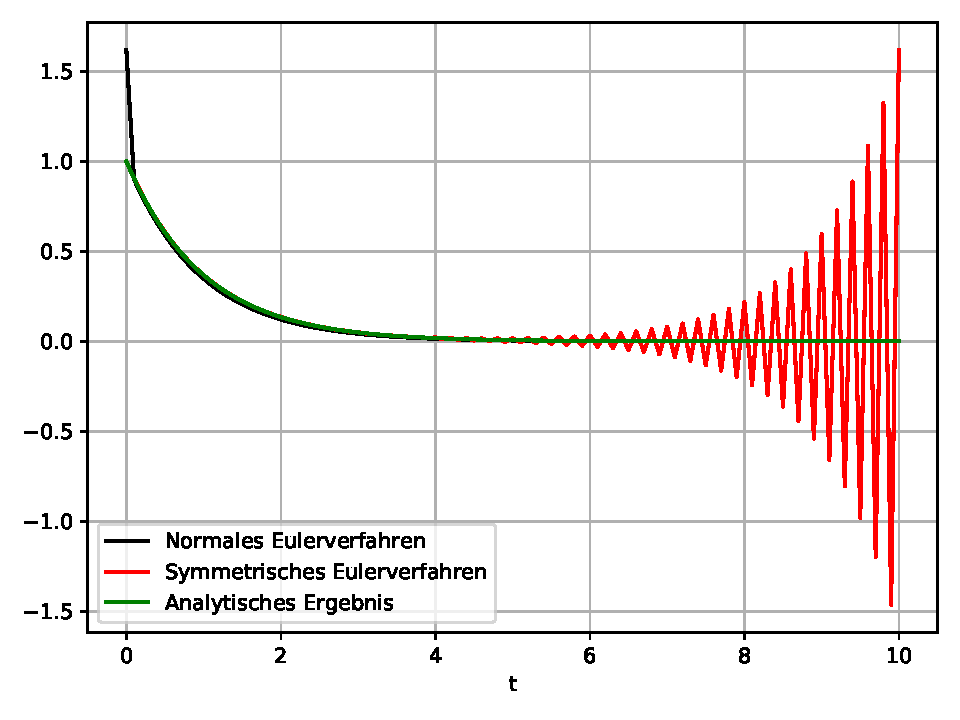
\includegraphics[height=8cm]{../../Blatt2/Plots/3.pdf}
  \caption{Laufzeit der unterschiedlichen Algorithmen in Nanosekunden in Abhängigkeit der Dimension N der Matrix.}
  \label{fig:laufzeit}
\end{figure}
Es lässt sich bei jedem Verfahren ein Potenzgesetz mit jeweils unterschiedlichem Exponenten erkennen.
Die LU Zerlegung mit nicht vollständiger Pivotisierung besitzt dabei stets die geringste Laufzeit, wohingegen insbesondere bei hohen N die LU Zerlegung mit vollständiger Pivotisierung am längsten dauert. Bei geringen N ist aber auch zum Teil die Methode mit Invertierung diejenige mit der längsten Laufzeit.

\subsection*{Aufgabenteil d)}
In Aufgabenteil c) hat sich gezeigt, dass die Methode mit nicht vollständer Pivotisierung für alle N am effizientesten ist. Bei Matrizen, bei denen sich die Elemente jedoch nicht stark unterscheiden kann es aufgrund von
Rundungsfehlern und Auslöschung zu großen Abweichungen und zu numerischer Instabilität führen, sodass in diesem Fall ein anderes Verfahren gewählt werden sollte. Ob dabei eine LU Zerlegung mit vollständiger Pivotisierung oder die Berechnung der Inversen effizienter ist hängt von der Dimension N ab. \\
Um diese Ergebnisse zu quantifizieren wird zudem der Exponent $a$ des jeweiligen Anstiegs der Laufzeit berechnet, indem die Laufzeit logarithmiert wird und eine lineare Ausgleichsrechnung der Form
\begin{equation}
  \text{ln}(\text{laufzeit})=a*\text{ln}(\text{N})+b
\end{equation}
mit ln(N) durchgeführt werden. Dabei werden nur Werte ab N$\geq2^5$ berücksichtigt, da erst ab hier im doppellogarithmischen Diagramm \ref{fig:laufzeit} eine Gerade zu erkennen ist. Dabei ergeben sich die Werte
\begin{align*}
  a_{inv}&= 2.58 \pm 0.07\\
  a_{full}&= 2.95 \pm 0.08\\
  a_{par}&= 2.56 \pm 0.06 \: ,
\end{align*}
woran sich erneut erkennen lässt, dass der Aufwand für die LU Zerlegung mit vollständiger Pivotisierung
bei großen N am stärksten ansteigt mit nahezu $\mathcal{O}(\text{N}^3)$. Die LU Zerlegung ohne vollständige Pivotisierung und die Inverse unterscheiden sich hingegen kaum im Exponenten, sondern stattdessen im Parameter $b$ mit Werten
\begin{align*}
  b_{inv}&= (2.7 \pm 0.4)\text{s} \\
  b_{full}&= (1.4 \pm 0.5)\text{s} \\
  b_{par}&= (1.6 \pm 0.4)\text{s} \: ,
\end{align*}
woran sich erkennen lässt, dass die Laufzeit der LU Zerlegung ohne vollständige Pivotisierung im Allgemeinen unter der, der Inversen liegt. Die Ausgleichsgeraden sind zudem in Abbildung \ref{fig:gerade} dargestellt.
\begin{figure}[H]
  \centering
  \includegraphics[height=8cm]{../../Blatt2/Plots/3_Geraden.pdf}
  \caption{Laufzeit der unterschiedlichen Algorithmen in Nanosekunden in Abhängigkeit der Dimension N der Matrix mit Ausgleichsgeraden für N$\geq2^5$.}
  \label{fig:gerade}
\end{figure}
